\chapter{Prueba de concepto}
\label{pruebaconcepto}

En este capítulo se va a hablar de una pequeña prueba de concepto que consiste en un escenario \ac{SDN}-\ac{NFV} donde todas las \acp{API} y herramientas mencionadas en los capítulos \ref{herramientas} y \ref{desarrollo} trabajan conjuntamente en total sintonía.

Inicialmente, se habla sobre el contexto en el que se ha enmarcado la prueba de concepto, haciendo especial referencia al proyecto Metro-Haul.

A continuación, se establece una arquitectura de desarrollo, en la que se define el papel de cada \ac{API} y herramienta, y como interactúan entre sí.

Por último, se realiza una explicación del funcionamiento de la prueba de concepto, así como una vista de los resultados finales.

\section{Contexto}
\label{sec:contexto}

Esta prueba de concepto está enmarcada dentro del proyecto europeo Metro-Haul\cite{metrohaulbib}. Su principal objetivo es el de diseñar arquitecturas de redes metro que sean accesibles para 5G, anticipándose a los posibles problemas futuros cuando 5G esté totalmente funcional en las redes de telecomunicación.

Estas nuevas arquitecturas aseguran que algunos parámetros de calidad de servicio, como la latencia o el \textit{jitter} sean lo más bajos posibles, así como una total integración de nuevas tecnologías referentes al campo de \ac{ICT}, como son \ac{SDN} y \ac{NFV}.

Para conseguir todos estos objetivos, Metro-Haul propone diferentes pruebas de concepto para demostrar nuevas soluciones referentes a la arquitectura de red utilizando las nuevas tecnologías para ir integrando paulatinamente la tecnología 5G.

\section{Arquitectura}
\label{sec:arquitectura}

El principal objetivo de la prueba de concepto es el de integrar todas las \acp{API} y herramientas mencionadas anteriormente para conseguir satisfacer diferentes \textit{Service Chains} con restricciones de latencia y ancho de banda. Además, se busca demostrar como todas las herramientas \textit{open-source} que componen dicha prueba de concepto trabajan en sintonía para crear un escenario \ac{SDN}-\ac{NFV} heterogéneo.

Para conseguir los objetivos mencionados anteriormente, se ha diseñado una arquitectura específica para poder llevar a cabo la prueba de concepto, donde cada uno de los elementos realiza una tarea en concreto.

\begin{figure}[!ht]
	\centering
	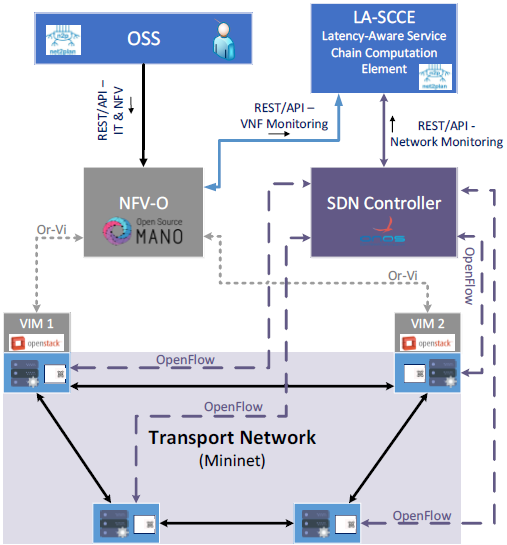
\includegraphics[width=0.9\linewidth]{imagenes/esquema_demo}
	\caption{Arquitectura de la Prueba de Concepto. Fuente:\cite{demoecocbib}}
	\label{fig:esquemademo}
\end{figure}

En la figura \ref{fig:esquemademo} se puede observar un esquema de la arquitectura, en el que se incluyen todos los elementos que la componen, y hace más fácil de entender como interactúan entre sí los componentes.

A continuación vemos una explicación de cada uno de los elementos que componen la prueba de concepto y que componente lleva a cabo esa acción:

\begin{itemize}
	\item \textbf{\ac{OSS}:} representa el papel de un operador que despliega un servicio gracias a una aplicación. El operador es emulado mediante Net2Plan, más concretamente por su plugin de \textit{NFV Management} (ver \ref{sec:nfvplugin}).
	
	\item \textbf{\ac{NFV-O}:} representa el papel de una aplicación que se encarga de gestionar la infraestructura de virtualización necesaria para instanciar diferentes máquinas virtuales. \ac{OSM} (ver \ref{sec:osm}) es el encargado de dicha función.
	
	\item \textbf{\acp{VIM}:} son los encargados de instanciar y alojar las diferentes máquinas virtuales pertenecientes a los VNF. OpenStack (ver \ref{sec:openstack}) es quien realiza este papel.
	
	\item \textbf{Red de Transporte:} la red de transporte es emulada mediante Mininet (ver \ref{sec:mininet}) para establecer flujos de paquetes entre las diferentes \acp{VNF} de una \textit{Service Chain}. La red se define mediante un script en Python (ver \ref{sec:scriptmininet}).
	
	\item \textbf{Controlador \ac{SDN}:} la red de transporte es controlada por una instancia de \ac{ONOS} (ver \ref{sec:onos}) mediante el envio de paquetes Openflow (ver \ref{subsec:openflow}) a los diferentes switches de la red.
	
	\item \textbf{\ac{LA-SCCE}:} Se encarga de decidir el camino a seguir para atravesar una secuencia de \acp{VNF} que cumpla con los requisitos de latencia máxima. Este papel lo representa la extensión de Net2Plan mediante la ejecución de un algoritmo de \textit{NFV Placement}. 
\end{itemize}


\section{Funcionamiento}
\label{sec:funcprueba}

Para llevar a cabo la prueba de concepto, la arquitectura explicada en la sección anterior se ha traducido en un \textit{testbed} para poder llevarla a cabo, como se puede apreciar en la figura \ref{fig:poctestbed}.

\begin{figure}[!ht]
	\centering
	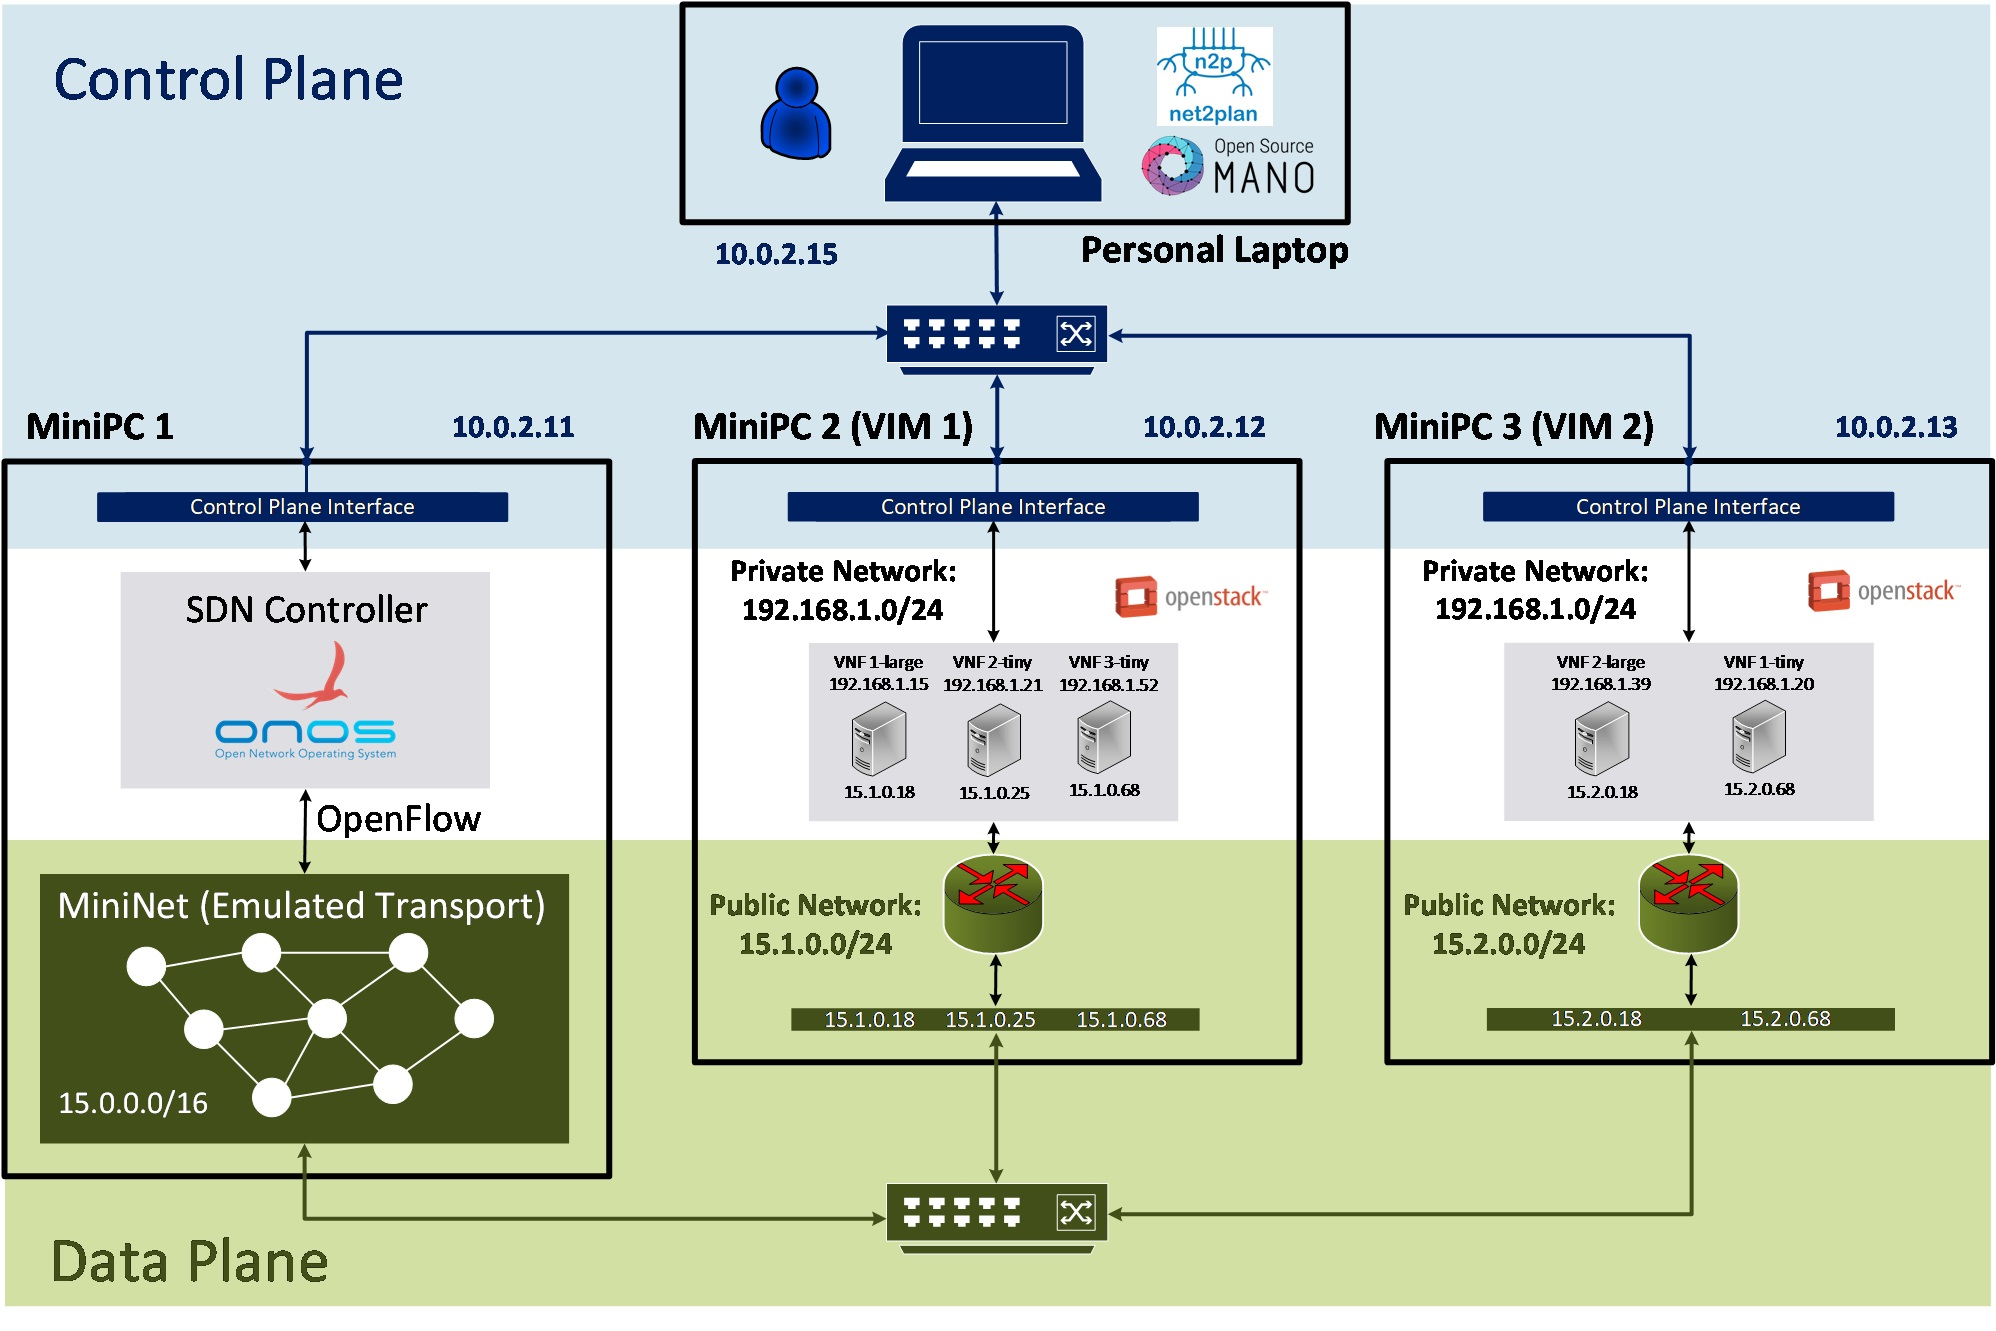
\includegraphics[width=0.9\linewidth]{imagenes/PoC_testbed}
	\caption{\textit{Testbed} para la Prueba de Concepto. Fuente:\cite{demoecocbib}}
	\label{fig:poctestbed}
\end{figure}

El \textit{testbed} montado se compone de cuatro \acp{PC} y dos \textit{switches}, uno para el plano de control y otro para el plano de datos:

\begin{itemize}
	\item \textbf{Mini\ac{PC}1:} Se encarga de alojar una instancia del controlador \ac{SDN} \ac{ONOS} y de emular la red de transporte gracias a Mininet.
	
	\item \textbf{Mini\ac{PC}2:} 
	
	\item \textbf{Mini\ac{PC}3:} 
	
	\item \textbf{\textit{Personal Laptop}:} 
\end{itemize}


A continuación se explican los diferentes pasos que se realizan para llevar a cabo la prueba de concepto y que APIs intervienen en cada uno de ellos:

\begin{figure}[!ht]
	\centering
	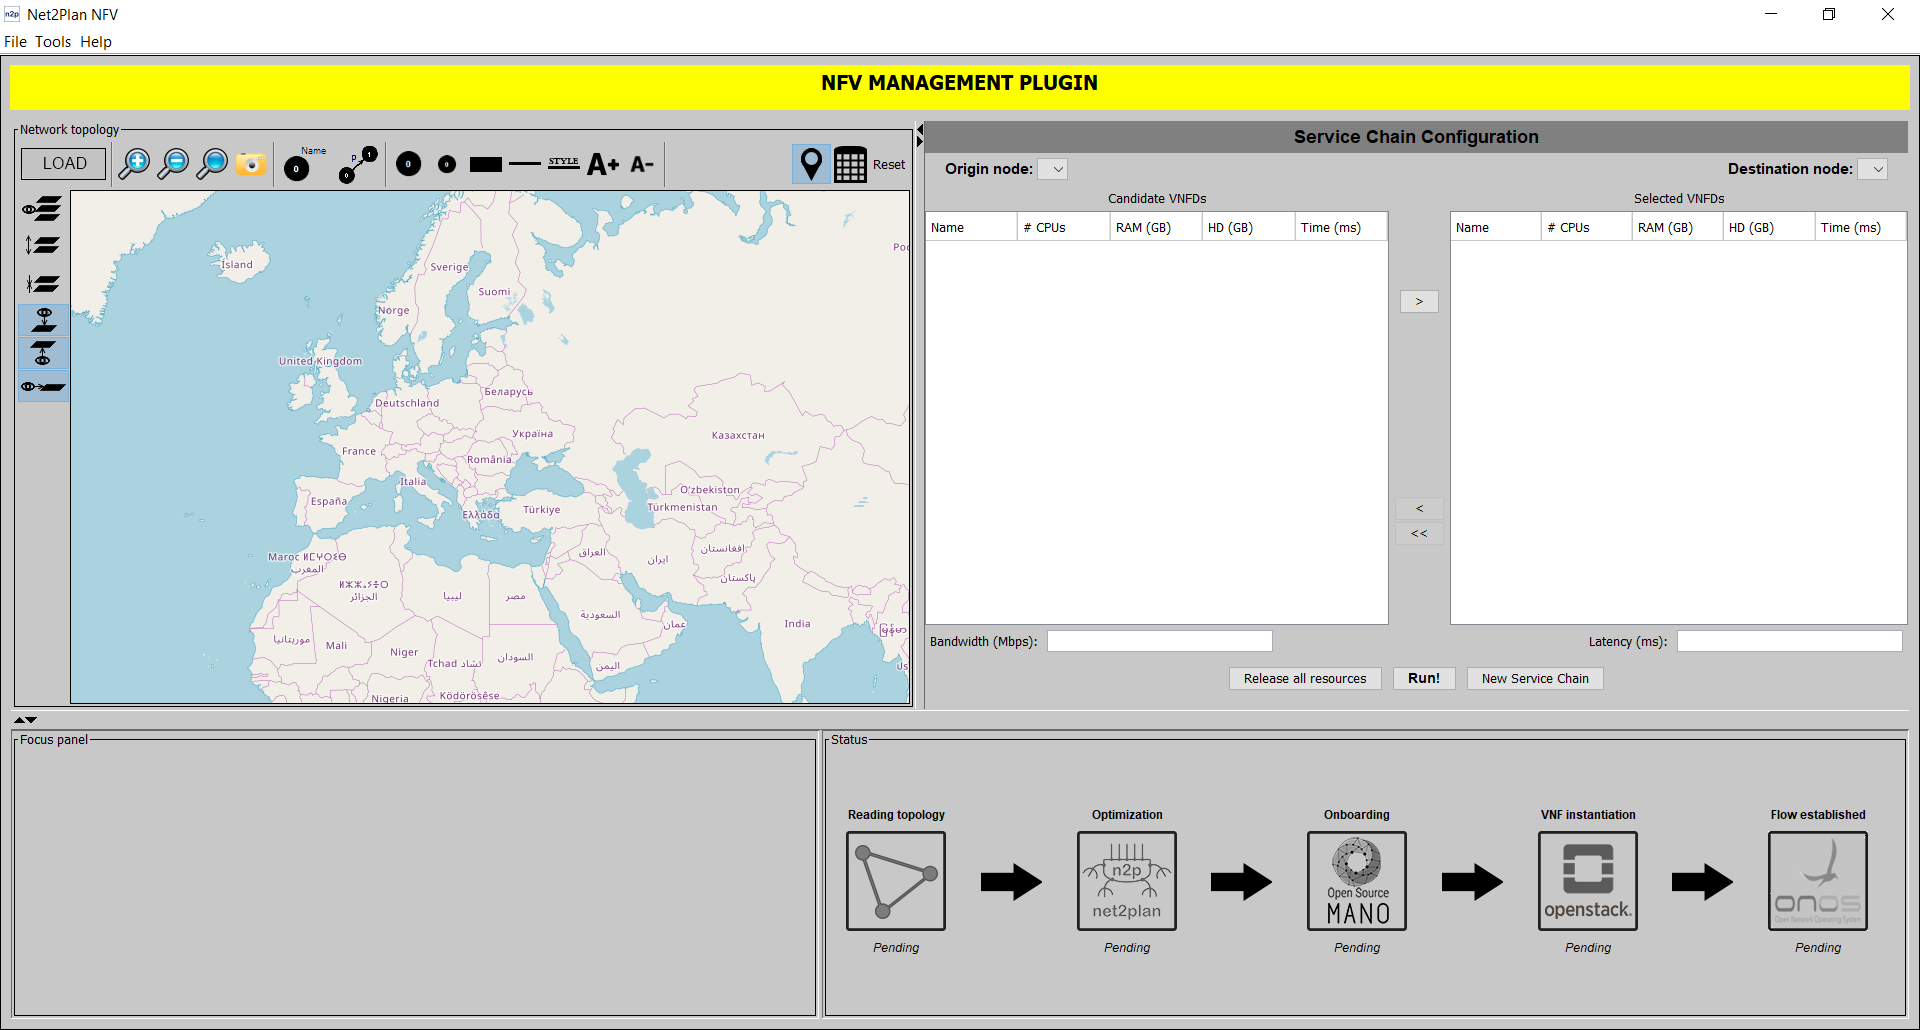
\includegraphics[width=0.9\linewidth]{imagenes/nfvplugin_dashboard}
	\caption{Interfaz gráfica del Plugin al inicio}
	\label{fig:nfvproof_inicio}
\end{figure}

\begin{itemize}
	\item Paso 1. Haciendo click en el botón LOAD, Net2Plan recibe la información referente a la red de transporte de ONOS haciendo uso de ONOSClient, la información sobre los posibles VNFs a instanciar de ETSI-OSM haciendo uso de J-OSMClient y la información sobre cada VIM de OpenStack haciendo uso de OpenStackClient.
	
	\item Paso 2. El usuario define la Service Chain que quiere satisfacer (nodo origen, nodo destino, secuencia ordenada de VNFs a atravesar, latencia máxima y ancho de banda) a través de la interfaz gráfica del Plugin.
	
	\item Paso 3. Net2Plan recibe la información introducida por el usuario y la transfiere al LA-SCCE para que ejecute el algoritmo que devolverá como resultado una ruta de enlaces para la Service Chain y una serie de VNFs instanciadas en diferentes VIMs.
	
		\begin{figure}[!ht]
		\centering
		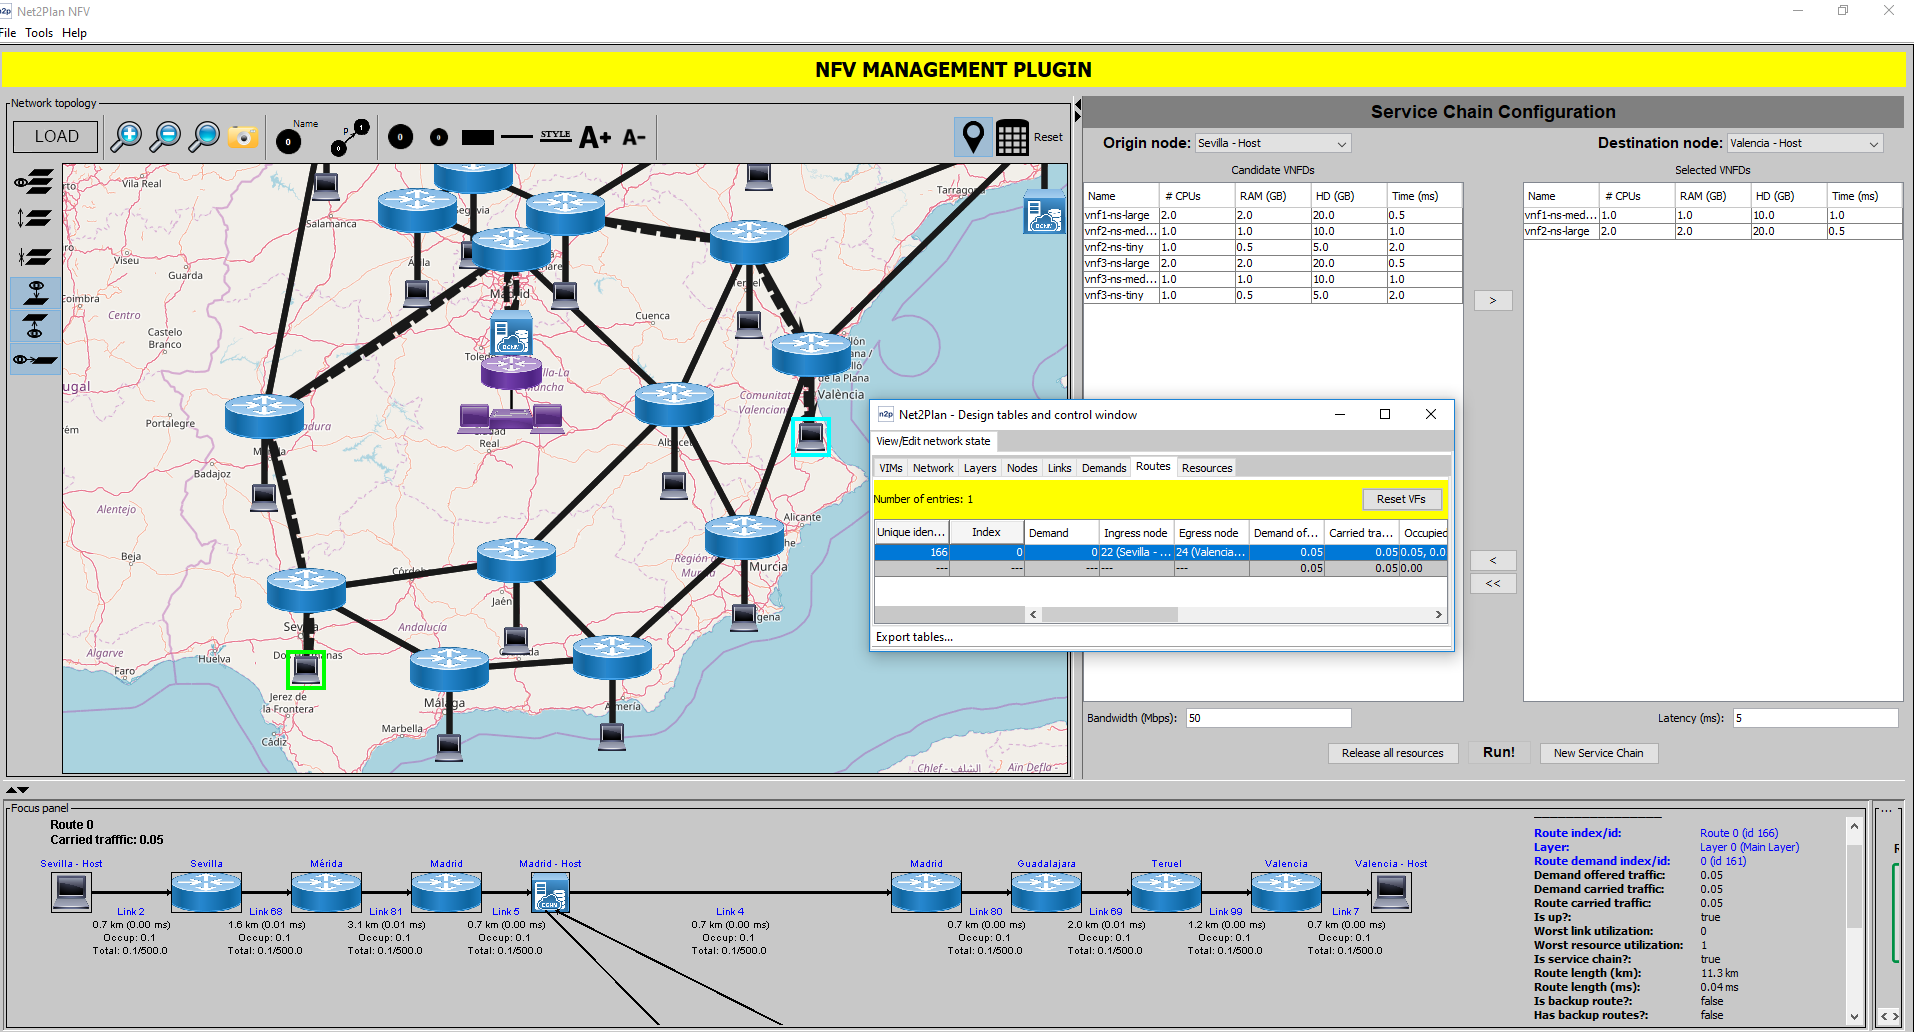
\includegraphics[width=0.9\linewidth]{imagenes/nfv_service_chain}
		\caption{Interfaz gráfica del Plugin con la ruta establecida}
		\label{fig:nfvservicechain}
	\end{figure}
	
	\item Paso 4. Net2Plan envía la orden a ETSI-OSM haciendo uso de J-OSMClient de instanciar las VNFs en los VIMs que el LA-SCCE obtuvo como óptimos.
	
	\begin{figure}[!ht]
		\centering
		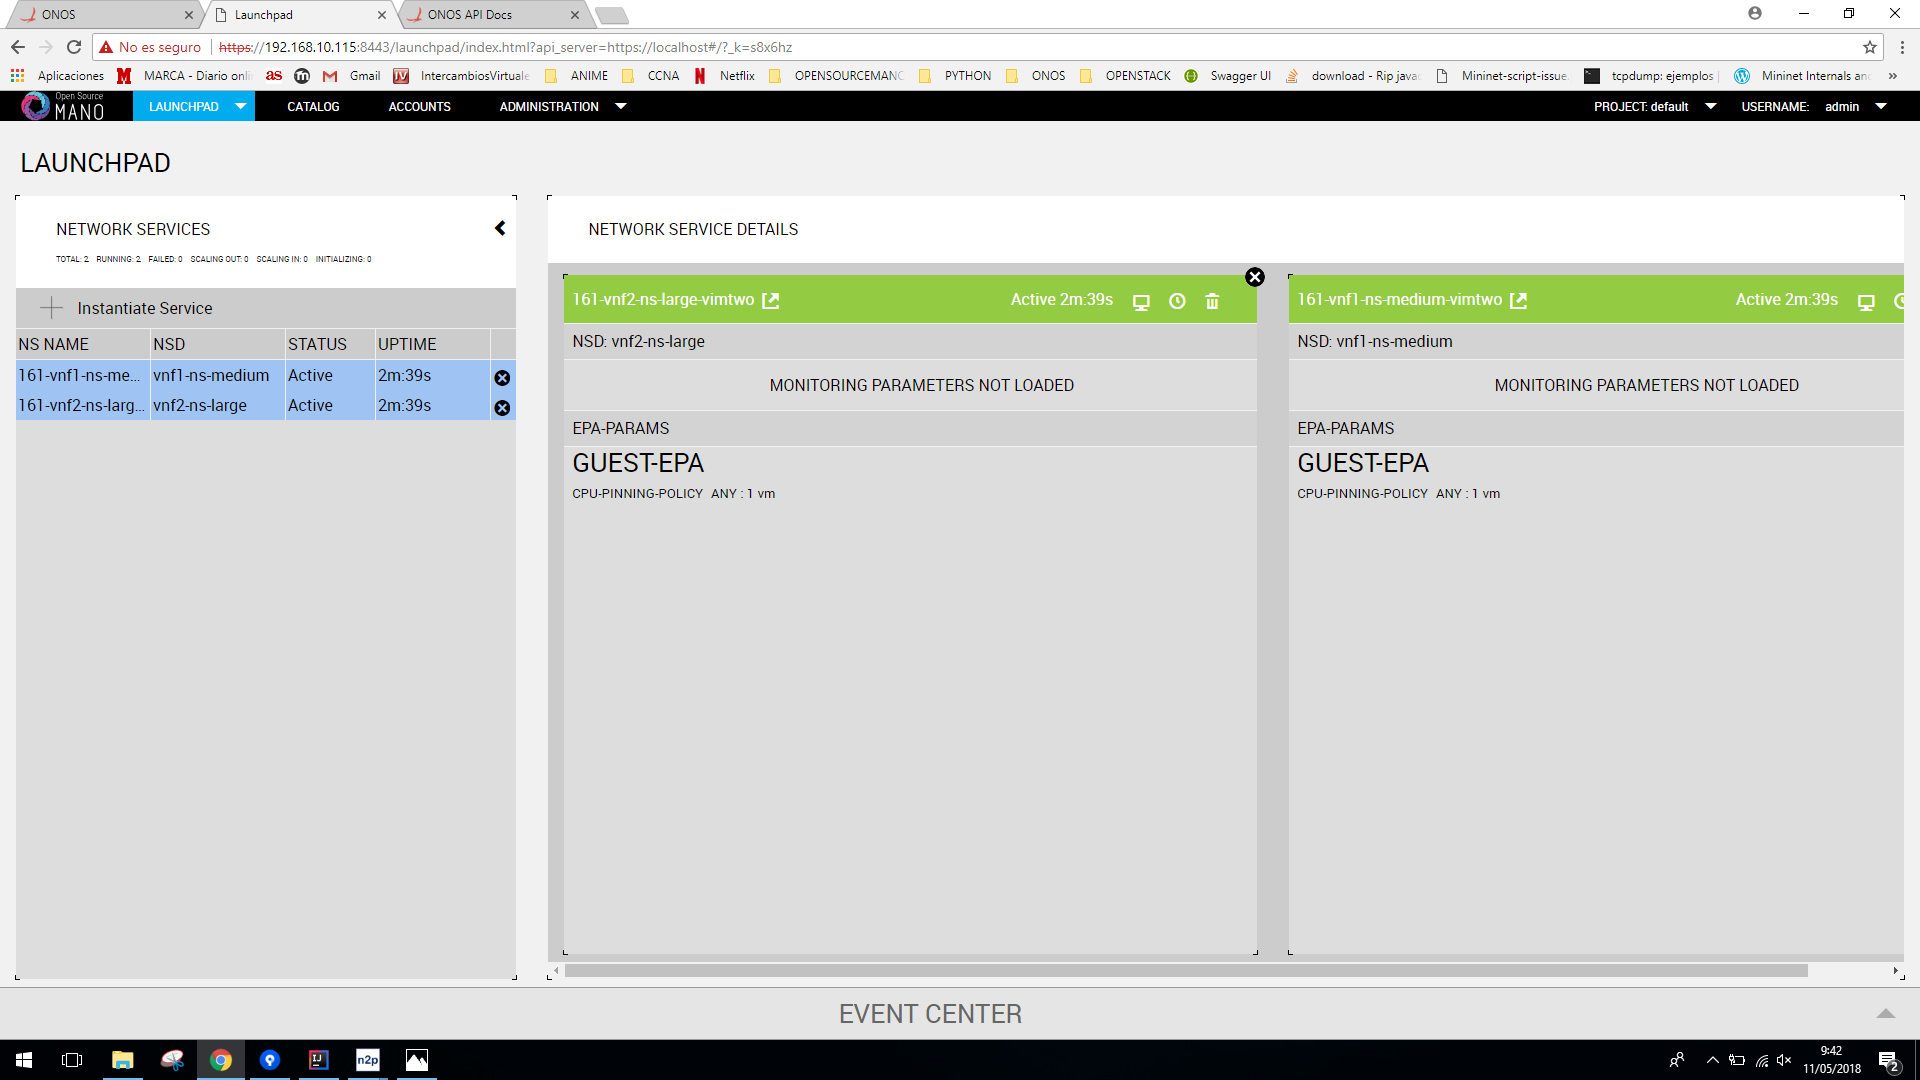
\includegraphics[width=0.9\linewidth]{imagenes/osm_vnfs}
		\caption{Interfaz gráfica de OSM con los VNFs instanciados}
		\label{fig:osmvnfs}
	\end{figure}
	
	
	\item Paso 5. ETSI-OSM envia órdenes a los diferentes VIMs (OpenStack) para que alojen las diferentes máquinas virtuales correspondientes a los VNFs. La comunicacion entre OSM y OpenStack es transparente al usuario.
	
	\item Paso 6. Net2Plan envía la orden a ONOS, haciendo uso de ONOSClient, con diferentes reglas de flujo para establecer en los diferentes switches de la red de transporte, todo según la ruta óptima obtenida por el LA-SCCE.
	
	\begin{figure}[!ht]
		\centering
		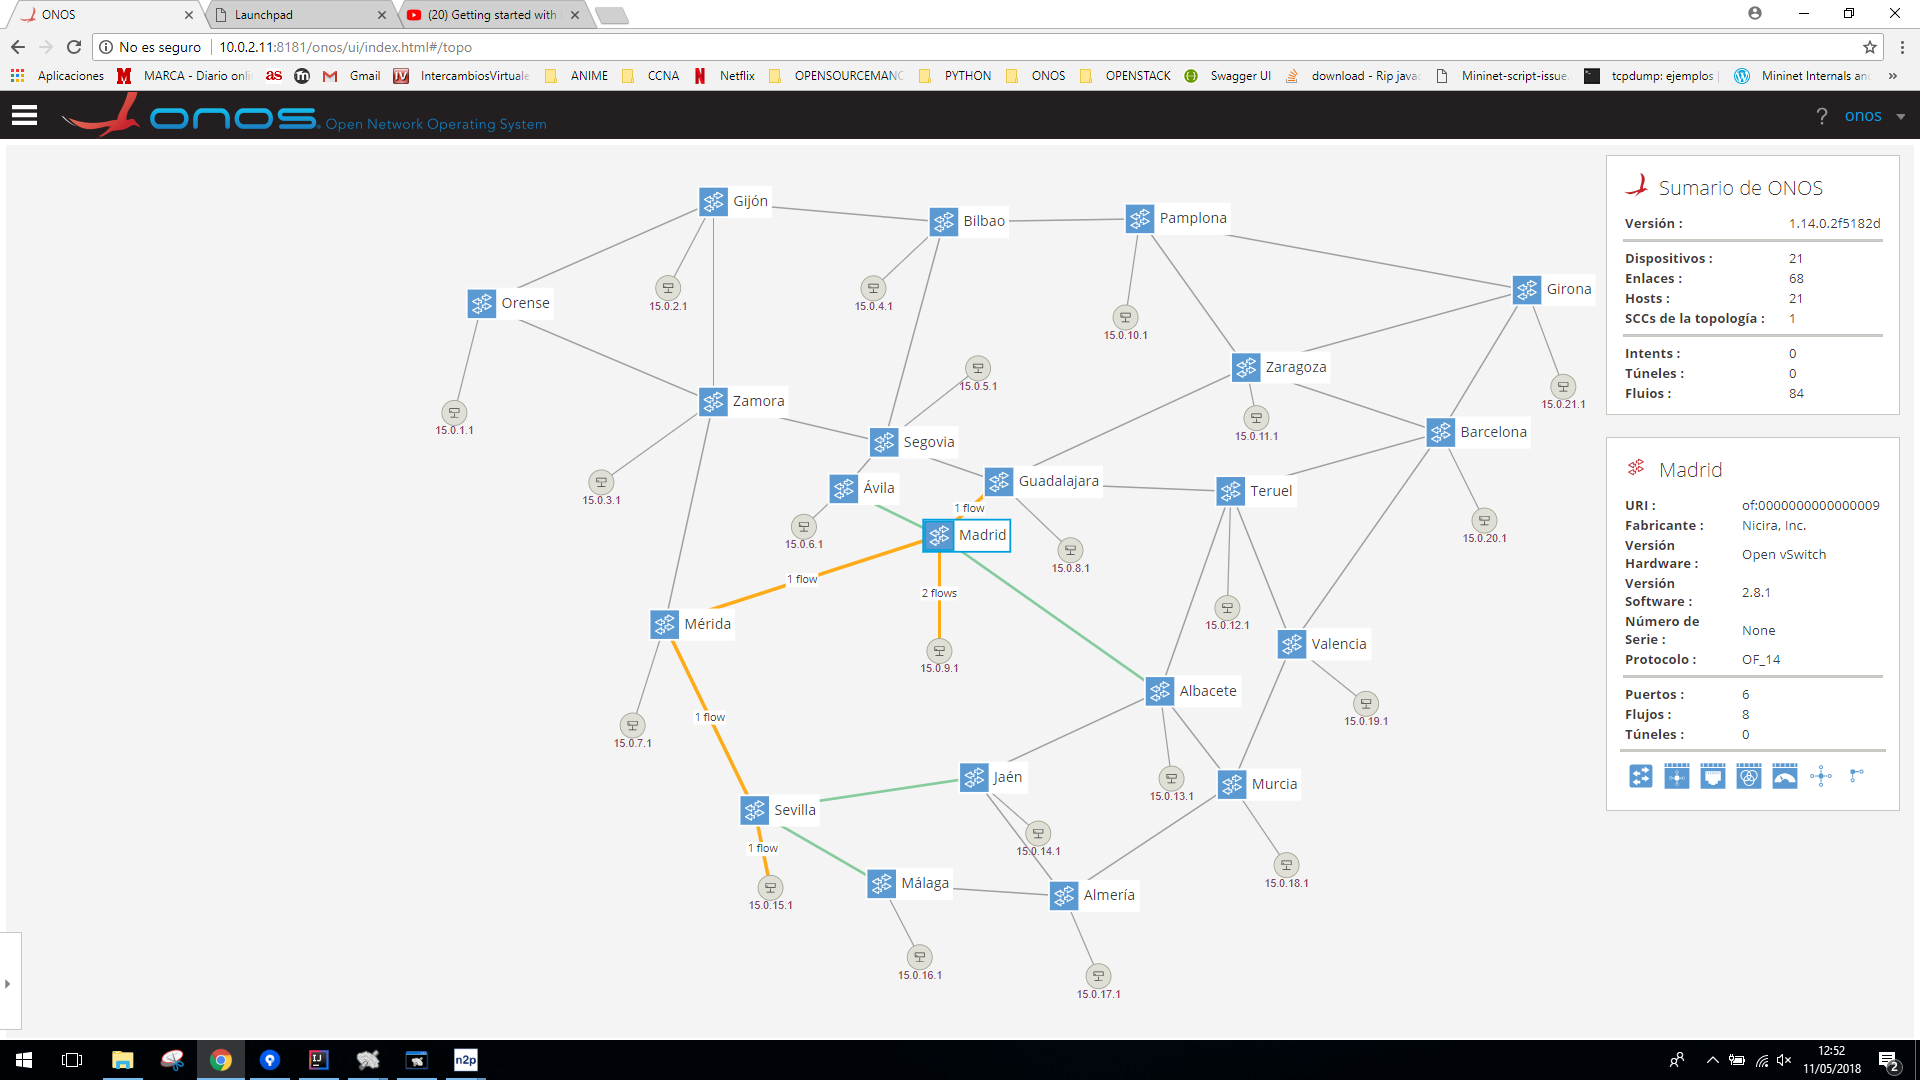
\includegraphics[width=0.9\linewidth]{imagenes/topo_onos}
		\caption{Interfaz gráfica de ONOS con las reglas de flujo establecidas}
		\label{fig:topo_onos}
	\end{figure}

	\item Paso 7. Una vez establecidos las reglas de flujo mediante OpenFlow, se realiza una prueba de conexión para asegurar que la Service Chain está establecida.
	
	\begin{figure}[!ht]
		\centering
		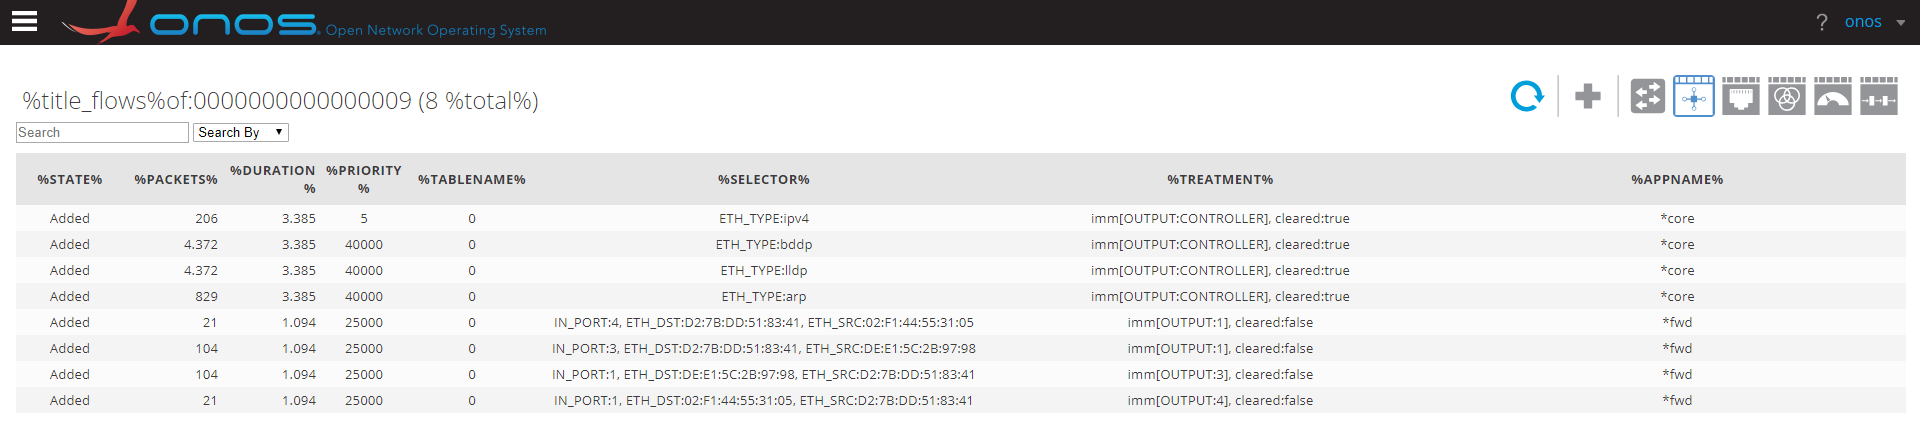
\includegraphics[width=0.9\linewidth]{imagenes/onos_flowrules}
		\caption{Prueba de conectividad en la GUI de ONOS}
		\label{fig:onosflowrules}
	\end{figure}


\end{itemize}

